\documentclass{beamer}
\usepackage{amsfonts,amsmath,oldgerm}
\usepackage{ragged2e}

\usetheme{sintef}

\newcommand{\testcolor}[1]{\colorbox{#1}{\textcolor{#1}{test}}~\texttt{#1}}

\usefonttheme[onlymath]{serif}

\titlebackground*{assets/background}

\newcommand{\hrefcol}[2]{\textcolor{cyan}{\href{#1}{#2}}}

\title{Aula 02 - História dos sistemas operacionais}
\subtitle{2023.1 - SPOSOPE - Sistemas Operacionais}
\course{Tecnologia em Análise e Desenvolvimento de Sistemas}
\author{\href{mailto:luizfpq@gmail.com}{Luiz \textbf{Quirino}}}
\IDnumber{luizfpq@gmail.com}



\begin{document}
\maketitle

%\begin{frame}
%
%      Este material é produzido utilizando \LaTeX\, baseado na SINTEF Presentation, disponibilizado sob licenciamento \hrefcol{https://creativecommons.org/licenses/by-nc/4.0/legalcode}{Creative Commons CC BY 4.0}
%
%\vspace{\baselineskip}

%In the following you find a brief introduction on how to use \LaTeX\ and the beamer package to prepare slides, based on the one written by \hrefcol{mailto:federico.zenith@sintef.no}{Federico Zenith} for \hrefcol{https://www.overleaf.com/latex/templates/sintef-presentation/jhbhdffczpnx}{SINTEF Presentation}

% This template is released under \hrefcol{https://creativecommons.org/licenses/by-nc/4.0/legalcode}{Creative Commons CC BY 4.0} license

%\end{frame}

\section{Sistemas monolíticos}

\begin{frame}{Sistemas Monolíticos}
    \begin{itemize}
        \item É a organização mais comum
        \item Poderia ser chamada de "A Grande Bagunça"
        \item Conjunto de rotinas que podem chamar umas
        as outras diretamente
        \item Cada rotina tem uma interface bem definida
        em termos de parâmetros e resultados
    \end{itemize}
\end{frame}
\begin{frame}{Sistemas Monolíticos - Compilação}
    \begin{itemize}
        \item Para construir o programa objeto todas as
        rotinas são compiladas individualmente (ou os
        arquivos que contém as rotinas)
        \item Depois esses arquivos são linkados em um
        único arquivo objeto
        \item Não existe ocultação de rotinas, toda rotina é
        visível para todas as outras
        \item Os pontos de entrada oficialmente designados
        podem ser chamados de fora dos módulos
    \end{itemize}
\end{frame}
\begin{frame}{SO Monolítico - Syscalls}
    \begin{itemize}
        \item Pode-se ter um pouco de estruturação
        \item Os serviços (syscalls) são solicitados colocando
        os parâmetros em locais bem definidos
        (registradores, pilha)
        \item Executamos então uma interrupção especial:
        \begin{itemize}
            \item Chamada de Núcleo ou de Supervisor
        \end{itemize}
    \end{itemize}
\end{frame}
\begin{frame}{SO Monolítico - Chama de Núcleo}
    \begin{itemize}
        \item Troca a máquina de modo usuário para modo núcleo
        \item Transfere o controle para o SO
        \item Dois modos de processadores (geralmente):
        \begin{itemize}
            \item Modo Núcleo: todas as instruções do ISA são permitidas
            \item Modo Usuário: algumas instruções do ISA são bloqueadas, geralmente de E/S
        \end{itemize}
    \end{itemize}
\end{frame}
\begin{frame}{SO Monolítico - Syscall}
    \begin{itemize}
        \item Exemplo: \texttt{count = read(fd, buffer, nbytes)}
        \item Faz a chamada de sistema \texttt{"read"}
        \item O programa insere os dados na pilha
        \item Detalhe: os compiladores C/C++ colocam os parâmetros de forma inversa na pilha
    \end{itemize}
\end{frame}
\begin{frame}{SO Monolítico - Estrutura Básica}
    \begin{enumerate}
        \item Um programa principal que ativa a função do serviço solicitada
        \item Um conjunto de funções de serviço que executam as chamadas do sistema
        \item Um conjunto de funções utilitárias que ajudam as funções de serviço
    \end{enumerate}
\end{frame}

\begin{frame}{SO Monolítico - Estrutura}
    \begin{itemize}
        \item Para cada syscall há uma função de serviço que cuida dela.
        \item Funções utilitárias fazem procedimentos necessários para as várias funções de serviço.
    \end{itemize}
\end{frame}


\section{Sistemas em Camadas}
\begin{frame}{Sistema em Camadas}
    \begin{itemize}
        \item O primeiro SO a implementar: THE
        \item THE (Technische Hogeschool Eindhoven)
        \item Holanda, 1968
        \item Construído por E. W. Dijistra e seus alunos
        \item Sistema em Lotes para o computador holandês Electrologica X8
        \item 32K de palavras de 27 bits
    \end{itemize}
\end{frame}
\begin{frame}{Sistema em Camadas}
    \begin{itemize}
        \item A camada acima nunca precisa se preocupar com o que está ocorrendo na camada de baixo.
        \item Camada 0: Alocação do processador, alternando entre processos quando ocorriam interrupção ou temporizadores expiravam.
        \item Camada 1: Gerenciamento de memória, alocando espaços para processos na memória principal e em um tambor (antigo meio magnético de armazenamento) com 512K.
        \item Camada 2: Manipulava a Comunicação entre Processos (IPC) e o console do operador.
    \end{itemize}
\end{frame}
\begin{frame}{Sistema em Camadas}
    \begin{itemize}
       
        \item Camada 3: Gerenciava dispositivos de E/S e armazenava em buffer os fluxos de informações.
        \item Camada 4: Os programas de usuário, não se preocupavam com gerenciamento algum (processos, memória, console ou E/S).
        \item Camada 5: Processo de operador do sistema.
    \end{itemize}
\end{frame}
\begin{frame}{Máquinas Virtuais}
    \begin{itemize}
        \item OS/360 = sistemas em lote.
        \item Muitos usuários do sistema queriam ter tempo compartilhado.
        \item Grupos dentro e fora da IBM decidiram escrever um sistema de tempo compartilhado para o OS/360.
        \item TSS/360 = tempo compartilhado oficial da IBM.
        \item Era grande e lento e foi abandonado, custando U\$50 milhões.
    \end{itemize}
\end{frame}
\begin{frame}{Máquinas Virtuais - VM/370}
    \begin{itemize}
        \item Um grupo científico da IBM em Cambridge desenvolveu outro sistema.
        \item Esse SO foi adotado pela IBM para computadores de grande porte.
        \item Originalmente chamava-se CP/M, mas depois foi renomeado para VM/370.
        \item Projetado com dois módulos principais:
              \begin{itemize}
                  \item Multiprogramação
                  \item Máquina Estendida
              \end{itemize}
    \end{itemize}
\end{frame}
\begin{frame}{Máquina Virtual - Monitor da VM}
    \begin{itemize}
        \item O centro do SO era conhecido como Monitor de Máquina Virtual.
        \item Executava-se no hardware básico e implementava a multiprogramação.
        \item Oferecia várias máquinas virtuais, que eram cópias exatas do hardware básico.
        \item Incluía os modos kernel e usuário, proporcionando isolamento e proteção entre as VMs.
        \item Preservava todos os detalhes originais da máquina real em cada VM.
    \end{itemize}
\end{frame}
\begin{frame}{Máquina Virtual}
    \begin{itemize}
        \item As máquinas virtuais podem executar sistemas operacionais distintos.
        \item Exemplo:
        \begin{itemize}
            \item Algumas VMs rodavam descendentes do OS/360 para processamento em lote.
            \item Outras executavam o CMS (Conversational Monitor System) para tempo compartilhado.
        \end{itemize}
        \item O conceito de máquinas virtuais também é empregado nos processadores compatíveis com x86, como o \textbf{Modo Virtual 8086}.
    \end{itemize}
\end{frame}


\section{modelo Cliente - Servidor}
\begin{frame}{Modelo Cliente-Servidor}
    \begin{itemize}
        \item Mover recursos do SO para fora do kernel.
        \item Deixando um núcleo mínimo: \textbf{Microkernel}.
        \item Implementar funções do SO como processos em modo usuário.
        \item Existe uma abordagem de processo cliente e processo servidor.
        \item O núcleo gerencia a comunicação entre clientes e servidores.
    \end{itemize}
\end{frame}
\begin{frame}{Modelo Cliente-Servidor}
    \begin{itemize}
        \item Os processos executando em modo usuário não têm acesso direto ao hardware.
        \item A consequência disso é que se ocorrer um erro no servidor de arquivos (por exemplo), não derrubará a máquina inteira.
        \item Capacidade de adaptação para uso em Sistemas Distribuídos.
    \end{itemize}
\end{frame}


\begin{frame}{Referências }\justifying
      \begin{itemize}
            \item \textbf{Slides SOPA2 - Prof. Alexandre Beletti Ferreira}
            \item \textbf{TANENBAUM, Andrew S.; WOODHULL, Albert S.} Sistemas operacionais: projeto e implementação. 3. ed. Porto Alegre: Bookman, 2008. ISBN 9788577800571.
      \end{itemize}
\end{frame}


\begin{frame}[fragile]{Imagem do dia}

    \begin{figure}[H]
        \centerline{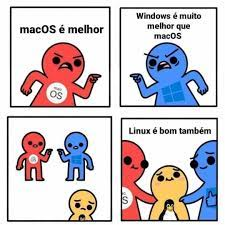
\includegraphics[width=0.4\textwidth]{assets/imagem-do-dia/sope-02.jpeg}}
        
    \end{figure}
\end{frame}

\backmatter
\end{document}
